\begin{enumerate}
    \item Not-Aus drücken!
    \item Ladedeckel öffnen
    \item Ladegerät anschließen
    \item Ladevorgang starten siehe \ref{sec: bilderanleitung_laden}
    \item Ladegerät abschließen \& Kabel in Ladebox verstauen
    \item Ladedeckel schließen
\end{enumerate}

\newpage
\section{Bilderanleitung Ladevorgang \label{sec: bilderanleitung_laden}}
Die Bedienung des Ladegerätes ist im Folgenden dargestellt: \\

In \autoref{fig:Ladegeraet_Hauptanzeige} lässt sich die Hauptanzeige des Ladegeräts erkennen, welche 
sofort erscheint, wenn die Akkus angeschlossen werden. 

\begin{figure}[H]
    \centering
    \includegraphics[width=.3\textwidth]{Fotos/Ladegereat/DSC_8742_Ladegereat_Hauptanzeige.png}
    \caption{Ladegerät Hauptanzeige \label{fig:Ladegeraet_Hauptanzeige}}
\end{figure}

Um in die Menüanzeige zu gelangen, müssen beide mittleren Touch-Buttons gedrückt werden.
Im nächsten Schritt ist der Modus \glqq Dual Task\grqq auszuwählen, siehe \autoref{fig:Ladegeraet_Menueanzeige}. Mit dem rechten mittleren Touch-Button lässt sich 
dieser Task auswählen. 
\begin{figure}[H]
    \centering
    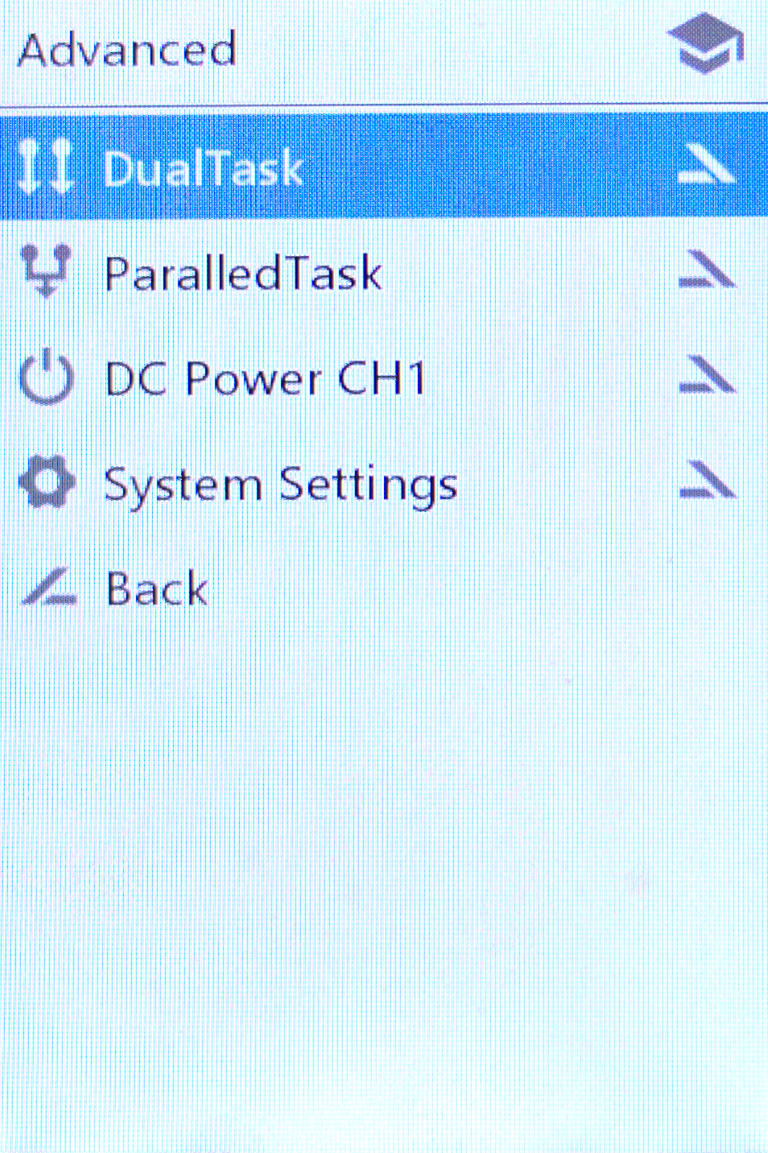
\includegraphics[width=.3\textwidth]{Fotos/Ladegereat/DSC_8744_Lademenue.png}
    \caption{Ladegerät Menüanzeige \label{fig:Ladegeraet_Menueanzeige}}
\end{figure}

Danach müssen die Parameter eingestellt werden wie in \autoref{fig:Ladegeraet_Menueanzeige2}. Mit den Touch-Buttons rechts oben oder unten lässt es sich durch das Menü 
scrollen und somit die richtige Einstellung auswählen. Nach dem fertigen Einstellen der Parameter, wird mit dem mittleren rechten Touch-Button auf \glqq Start\grqq gedrückt. 
\begin{figure}[H]
    \centering
    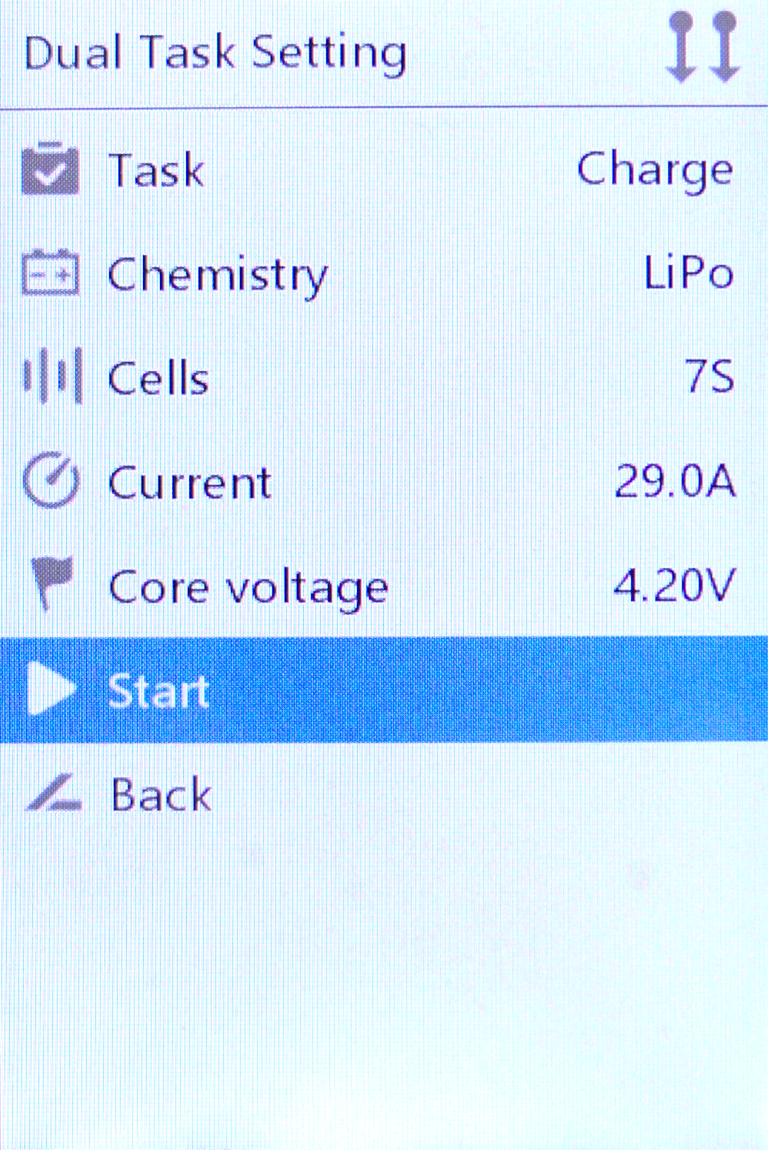
\includegraphics[width=.3\textwidth]{Fotos/Ladegereat/DSC_8745_Lademenue_2.png}
    \caption{Ladegerät Menüanzeige 2 \label{fig:Ladegeraet_Menueanzeige2}}
\end{figure}

In \autoref{fig:Ladegeraet_Ladezustand} lässt sich erkennen, wie das Display des Ladegeräts während dem Ladevorgang ausschaut.
Das Ladegerät piepst wenn der Ladevorgang beendet ist. 
\begin{figure}[H]
    \centering
    \includegraphics[width=.3\textwidth]{Fotos/Ladegereat/DSC_8747_Laden.png}
    \caption{Ladegerät Ladezustand \label{fig:Ladegeraet_Ladezustand}}
\end{figure}

 \todo{das zu einer section machen?}